\documentclass[3p]{elsarticle}
%DIF LATEXDIFF DIFFERENCE FILE
%DIF DEL _base16.tex                       Thu Oct 15 14:20:19 2026
%DIF ADD solderbench_softwarex_draft.tex   Thu Oct 15 14:26:09 2026
\usepackage{times}
\usepackage{graphicx}
\graphicspath{{figures/}}
\usepackage{booktabs}
\usepackage{amsmath}
\usepackage{xurl}
\def\UrlBreaks{\do\/\do\.\do\-}
\usepackage[pdfencoding=auto]{hyperref}
\hypersetup{colorlinks=true,urlcolor=blue}
%DIF PREAMBLE EXTENSION ADDED BY LATEXDIFF
%DIF UNDERLINE PREAMBLE %DIF PREAMBLE
\RequirePackage[normalem]{ulem} %DIF PREAMBLE
\RequirePackage{color}\definecolor{RED}{rgb}{1,0,0}\definecolor{BLUE}{rgb}{0,0,1} %DIF PREAMBLE
\providecommand{\DIFaddtex}[1]{{\protect\color{blue}\uwave{#1}}} %DIF PREAMBLE
\providecommand{\DIFdeltex}[1]{{\protect\color{red}\sout{#1}}} %DIF PREAMBLE
%DIF SAFE PREAMBLE %DIF PREAMBLE
\providecommand{\DIFaddbegin}{} %DIF PREAMBLE
\providecommand{\DIFaddend}{} %DIF PREAMBLE
\providecommand{\DIFdelbegin}{} %DIF PREAMBLE
\providecommand{\DIFdelend}{} %DIF PREAMBLE
\providecommand{\DIFmodbegin}{} %DIF PREAMBLE
\providecommand{\DIFmodend}{} %DIF PREAMBLE
%DIF FLOATSAFE PREAMBLE %DIF PREAMBLE
\providecommand{\DIFaddFL}[1]{\DIFadd{#1}} %DIF PREAMBLE
\providecommand{\DIFdelFL}[1]{\DIFdel{#1}} %DIF PREAMBLE
\providecommand{\DIFaddbeginFL}{} %DIF PREAMBLE
\providecommand{\DIFaddendFL}{} %DIF PREAMBLE
\providecommand{\DIFdelbeginFL}{} %DIF PREAMBLE
\providecommand{\DIFdelendFL}{} %DIF PREAMBLE
%DIF HYPERREF PREAMBLE %DIF PREAMBLE
\providecommand{\DIFadd}[1]{\texorpdfstring{\DIFaddtex{#1}}{#1}} %DIF PREAMBLE
\providecommand{\DIFdel}[1]{\texorpdfstring{\DIFdeltex{#1}}{}} %DIF PREAMBLE
\providecommand{\DIFscaledelfig}{0.5}
%DIF HIGHLIGHTGRAPHICS PREAMBLE %DIF PREAMBLE
\RequirePackage{settobox} %DIF PREAMBLE
\RequirePackage{letltxmacro} %DIF PREAMBLE
\newsavebox{\DIFdelgraphicsbox} %DIF PREAMBLE
\newlength{\DIFdelgraphicswidth} %DIF PREAMBLE
\newlength{\DIFdelgraphicsheight} %DIF PREAMBLE
% store original definition of \includegraphics %DIF PREAMBLE
\LetLtxMacro{\DIFOincludegraphics}{\includegraphics} %DIF PREAMBLE
\providecommand{\DIFaddincludegraphics}[2][]{{\color{blue}\fbox{\DIFOincludegraphics[#1]{#2}}}} %DIF PREAMBLE
\providecommand{\DIFdelincludegraphics}[2][]{% %DIF PREAMBLE
\sbox{\DIFdelgraphicsbox}{\DIFOincludegraphics[#1]{#2}}% %DIF PREAMBLE
\settoboxwidth{\DIFdelgraphicswidth}{\DIFdelgraphicsbox} %DIF PREAMBLE
\settoboxtotalheight{\DIFdelgraphicsheight}{\DIFdelgraphicsbox} %DIF PREAMBLE
\scalebox{\DIFscaledelfig}{% %DIF PREAMBLE
\parbox[b]{\DIFdelgraphicswidth}{\usebox{\DIFdelgraphicsbox}\\[-\baselineskip] \rule{\DIFdelgraphicswidth}{0em}}\llap{\resizebox{\DIFdelgraphicswidth}{\DIFdelgraphicsheight}{% %DIF PREAMBLE
\setlength{\unitlength}{\DIFdelgraphicswidth}% %DIF PREAMBLE
\begin{picture}(1,1)% %DIF PREAMBLE
\thicklines\linethickness{2pt} %DIF PREAMBLE
{\color[rgb]{1,0,0}\put(0,0){\framebox(1,1){}}}% %DIF PREAMBLE
{\color[rgb]{1,0,0}\put(0,0){\line( 1,1){1}}}% %DIF PREAMBLE
{\color[rgb]{1,0,0}\put(0,1){\line(1,-1){1}}}% %DIF PREAMBLE
\end{picture}% %DIF PREAMBLE
}\hspace*{3pt}}} %DIF PREAMBLE
} %DIF PREAMBLE
\LetLtxMacro{\DIFOaddbegin}{\DIFaddbegin} %DIF PREAMBLE
\LetLtxMacro{\DIFOaddend}{\DIFaddend} %DIF PREAMBLE
\LetLtxMacro{\DIFOdelbegin}{\DIFdelbegin} %DIF PREAMBLE
\LetLtxMacro{\DIFOdelend}{\DIFdelend} %DIF PREAMBLE
\DeclareRobustCommand{\DIFaddbegin}{\DIFOaddbegin \let\includegraphics\DIFaddincludegraphics} %DIF PREAMBLE
\DeclareRobustCommand{\DIFaddend}{\DIFOaddend \let\includegraphics\DIFOincludegraphics} %DIF PREAMBLE
\DeclareRobustCommand{\DIFdelbegin}{\DIFOdelbegin \let\includegraphics\DIFdelincludegraphics} %DIF PREAMBLE
\DeclareRobustCommand{\DIFdelend}{\DIFOaddend \let\includegraphics\DIFOincludegraphics} %DIF PREAMBLE
\LetLtxMacro{\DIFOaddbeginFL}{\DIFaddbeginFL} %DIF PREAMBLE
\LetLtxMacro{\DIFOaddendFL}{\DIFaddendFL} %DIF PREAMBLE
\LetLtxMacro{\DIFOdelbeginFL}{\DIFdelbeginFL} %DIF PREAMBLE
\LetLtxMacro{\DIFOdelendFL}{\DIFdelendFL} %DIF PREAMBLE
\DeclareRobustCommand{\DIFaddbeginFL}{\DIFOaddbeginFL \let\includegraphics\DIFaddincludegraphics} %DIF PREAMBLE
\DeclareRobustCommand{\DIFaddendFL}{\DIFOaddendFL \let\includegraphics\DIFOincludegraphics} %DIF PREAMBLE
\DeclareRobustCommand{\DIFdelbeginFL}{\DIFOdelbeginFL \let\includegraphics\DIFdelincludegraphics} %DIF PREAMBLE
\DeclareRobustCommand{\DIFdelendFL}{\DIFOaddendFL \let\includegraphics\DIFOincludegraphics} %DIF PREAMBLE
%DIF AMSMATHULEM PREAMBLE %DIF PREAMBLE
\makeatletter %DIF PREAMBLE
\let\sout@orig\sout %DIF PREAMBLE
\renewcommand{\sout}[1]{\ifmmode\text{\sout@orig{\ensuremath{#1}}}\else\sout@orig{#1}\fi} %DIF PREAMBLE
\makeatother %DIF PREAMBLE
%DIF COLORLISTINGS PREAMBLE %DIF PREAMBLE
\RequirePackage{listings} %DIF PREAMBLE
\RequirePackage{color} %DIF PREAMBLE
\lstdefinelanguage{DIFcode}{ %DIF PREAMBLE
%DIF DIFCODE_UNDERLINE %DIF PREAMBLE
  moredelim=[il][\color{red}\sout]{\%DIF\ <\ }, %DIF PREAMBLE
  moredelim=[il][\color{blue}\uwave]{\%DIF\ >\ } %DIF PREAMBLE
} %DIF PREAMBLE
\lstdefinestyle{DIFverbatimstyle}{ %DIF PREAMBLE
	language=DIFcode, %DIF PREAMBLE
	basicstyle=\ttfamily, %DIF PREAMBLE
	columns=fullflexible, %DIF PREAMBLE
	keepspaces=true %DIF PREAMBLE
} %DIF PREAMBLE
\lstnewenvironment{DIFverbatim}[1][]{\lstset{style=DIFverbatimstyle}}{} %DIF PREAMBLE
\lstnewenvironment{DIFverbatim*}[1][]{\lstset{style=DIFverbatimstyle,showspaces=true}}{} %DIF PREAMBLE
\lstset{extendedchars=\true,inputencoding=utf8}

%DIF END PREAMBLE EXTENSION ADDED BY LATEXDIFF

\begin{document}
\begin{frontmatter}
\title{Solderbench: An open-source synthetic benchmark for PCB solder-joint defect inspection algorithm development}
\author[1]{Qinmin Wang\fnref{fn1}}
\author[2]{Zixin Wang\fnref{fn2}}
\author[1]{Hongyuan Wang}
\author[3]{Zongzhong Wang\corref{cor1}}
\address[1]{School of Computer Science and Artificial Intelligence, Guangdong University of Science and Technology, Dongguan, China}
\address[2]{School of Electronic and Communication Engineering, Tianjin Normal University, Tianjin, China}
\address[3]{School of Electromechanical Engineering, Guangdong University of Technology, Guangzhou, China}
\cortext[cor1]{Corresponding author at School of Electromechanical Engineering, Guangdong University of Technology, Guangzhou, China. E-mail: wangzz@gdut.edu.cn}
\fntext[fn1]{E-mail: wangqinmin@gdust.edu.cn}
\fntext[fn2]{E-mail: 396514839@qq.com}
\begin{abstract}
Automated optical inspection (AOI) of solder joints is a critical quality-control step in printed circuit board (PCB) assembly, and three-dimensional (3D) point-cloud inspection is increasingly adopted because solder quality is essentially a volumetric property. However, publicly available 3D solder-joint datasets are essentially nonexistent: industrial scan data are proprietary, so new inspection algorithms are difficult to compare fairly. We present Solderbench, an open-source, pure-Python synthetic benchmark for developing and evaluating 3D solder-joint defect inspection algorithms. Solderbench provides (i) a parametric point-cloud generator that simulates five joint classes (good, insufficient, excessive, bridging, and collapse) with more than fifteen controllable parameters and \mbox{seed-level}, point-wise reproducibility; (ii) a seven-dimensional geometric feature extractor; (iii) six baseline classifiers, including \DIFdelbegin \DIFdel{a re-implementation of the industrial volume-threshold rule }\DIFdelend \DIFaddbegin \DIFadd{the original rule-based }\DIFaddend S3DA \DIFaddbegin \DIFadd{volume-threshold algorithm}\DIFaddend ; and (iv) automated comparison and ablation runners that export CSV, LaTeX, and figure artifacts. On a 1250-sample benchmark (seed 42), a random forest reaches 0.9440 accuracy and 0.9439 macro-$F_1$\DIFdelbegin \DIFdel{, and feature }\DIFdelend \DIFaddbegin \DIFadd{; multi-seed repeated experiments (five independent seeds) yield a mean test accuracy of $0.9531 \pm 0.0115$ for the random forest. Feature }\DIFaddend ablation identifies height variance as the most informative descriptor. Synthetic results serve as a controlled, reproducible proxy for algorithm development, yet final validation must be performed using real-world production scan data.
\end{abstract}
\begin{keyword}
solder joint inspection; automated optical inspection; 3D point cloud; synthetic benchmark; defect classification; reproducible evaluation; PCB; synthetic dataset
\end{keyword}
\end{frontmatter}
\section{Required metadata}
%DIF <  C2/C3/C8 filled: GitHub = https://github.com/wqinmin975/pcb ; Zenodo DOI = 10.5281/zenodo.22959193 (v0.1.1).
%DIF >  C2/C3/C8 filled: GitHub = https://github.com/wqinmin975/pcb ; Zenodo concept DOI = 10.5281/zenodo.22959192 (resolves to the latest release, v0.1.3).
\begin{table}[htbp]
\centering
\caption{Code metadata (mandatory).}
\begin{tabular}{lp{0.40\linewidth}p{0.46\linewidth}}
\toprule
\textbf{Nr.} & \textbf{Code metadata description} & \textbf{Value} \\
\midrule
C1 & Current code version & v0.1\DIFdelbeginFL \DIFdelFL{.1 }\DIFdelendFL \DIFaddbeginFL \DIFaddFL{.3 }\DIFaddendFL \\
C2 & Permanent link to code/repository used for this code version & \url{https://github.com/wqinmin975/pcb} \\
C3 & Permanent link to reproducible capsule & \DIFdelbeginFL %DIFDELCMD < \url{10.5281/zenodo.22959193} %%%
\DIFdelendFL \DIFaddbeginFL \url{https://doi.org/10.5281/zenodo.22959192} \DIFaddFL{(concept DOI, resolves to the latest release; v0.1.1 version DOI: }\url{https://doi.org/10.5281/zenodo.22959193}\DIFaddFL{) }\DIFaddendFL \\
C4 & Legal code license & MIT License \\
C5 & Code versioning system used & git \\
C6 & Software code languages, tools, and services used & Python ($\ge$ 3.8) \\
C7 & Compilation requirements, operating environments and dependencies & NumPy, SciPy, pandas, scikit-learn, and Matplotlib; OS-independent (no compilation, no GPU required) \\
C8 & Link to developer documentation/manual & \url{https://github.com/wqinmin975/pcb\#readme} \\
C9 & Support email for questions & wangzz@gdut.edu.cn \\
\bottomrule
\end{tabular}
\end{table}
\section{Motivation and significance}
Surface-mount technology (SMT) dominates modern printed-circuit-board (PCB) assembly, and solder-joint quality largely determines product reliability. AOI is the standard quality-control step on SMT lines \cite{ref1,ref2,ref3}; classical 2D AOI and deep-learning 2D detectors \cite{ref4} on public datasets such as DeepPCB \cite{ref5} are mature, yet inspection is increasingly moving to 3D because solder quality is fundamentally volumetric \cite{ref6,ref7}. General 3D deep learning (PointNet/PointNet++ \cite{ref8,ref9}, Open3D \cite{ref10}) has advanced, but 3D solder-joint research remains hampered by the absence of public data: existing public PCB datasets are almost entirely 2D \cite{ref5}, and the few 3D studies rely on private, non-public in-house point-cloud datasets \cite{ref6,ref7}, so algorithms cannot be compared fairly or reproduced. Solderbench closes this gap synthetically, simulating solder-joint point clouds from a parametric geometric model whose parameters (nominal joint size, noise, defect strength, bridging distance, collapse depth) are physically interpretable and user-controllable; synthetic generation yields costless labeled data of arbitrary size, deliberate control of class difficulty and sensor noise, and seed-level reproducibility.
\section{Software description}
\subsection{Software architecture}
Solderbench is a pure-Python package (about 1,000 source lines) with five feed-forward modules behind one public API: \texttt{generator.py} (parametric simulator), \texttt{features.py} (seven descriptors), \texttt{baselines.py} (six classifiers), \texttt{evaluate.py} (\texttt{run\_comparison}/\texttt{run\_ablation} runners exporting CSV, Booktabs-style LaTeX tables, and figures), and \texttt{data.py} (\texttt{load\_dataset()}, the real-camera integration point). Stages exchange NumPy arrays and pandas DataFrames, so any stage is replaceable; synthetic clouds swap for segmented real scans at \texttt{load\_dataset()} without downstream changes. The package ships a 15-test suite (shape and class-balance checks, same-seed reproducibility, feature validity, a Welch $t$-test that insufficient-solder volumes are significantly smaller, and fit-and-predict smoke tests), a \texttt{pyproject.toml}, and a \texttt{codemeta.json}; dependencies are only NumPy, SciPy, pandas, scikit-learn, and Matplotlib \cite{ref14,ref15,ref16,ref17}. All results use the versions pinned in \texttt{requirements.txt} (scikit-learn 1.9.0, NumPy 2.5.2, pandas 3.0.6, SciPy 1.18.0, Matplotlib 3.11.1; Python 3.13); the benchmark is fully deterministic from seed 42, so \texttt{python examples/run\_benchmark.py} regenerates every table and figure. \DIFaddbegin \textbf{\DIFadd{Note on real-world input:}} \texttt{\DIFadd{load\_dataset()}} \DIFadd{provides a software hook for external real-world point-cloud input. Real-world data acquisition, joint segmentation and pre-processing functions are }\emph{\DIFadd{not}} \DIFadd{implemented within this package; users must supply pre-segmented solder-joint point clouds (or their own }\texttt{\DIFadd{X, y}} \DIFadd{feature matrix) at this hook, after which every downstream experiment runs unchanged.
}\DIFaddend \subsection{Software functionalities}
\textbf{Generation. }SolderJointGenerator simulates five SMT defect classes \cite{ref6,ref7}: good, insufficient (shrunk ellipsoid, 0.55--0.85 of nominal), excessive (inflated ellipsoid, mean inflation 1.3, plus a bump), bridging (small center-to-center distance plus a strip), and collapse (random top dent). Over fifteen parameters control $n_{\mathrm{points}}$, noise, and the shrinkage, inflation, bridging, and collapse ranges; class ranges deliberately overlap so no classifier is perfect, and difficulty is tuned by widening or narrowing them. \DIFaddbegin \textbf{\DIFadd{Table~\ref{tab:params}}} \DIFadd{lists all generator parameters with their defaults and physical meaning.
}\DIFaddend 

\DIFaddbegin \begin{table}[htbp]
\centering
\caption{\DIFaddFL{Configurable parameters of }\texttt{\DIFaddFL{SolderJointGenerator}} \DIFaddFL{(defaults used for every reported result; all spatial quantities in mm).}}
\label{tab:params}
\renewcommand{\arraystretch}{1.12}
{\small
\begin{tabular}{@{}p{0.28\linewidth}p{0.11\linewidth}p{0.55\linewidth}@{}}
\toprule
\textbf{Parameter} & \textbf{Default} & \textbf{Physical meaning} \\
\midrule
\texttt{n\_points} & 1500 & fixed point count per cloud (simulates scanner resolution) \\
\texttt{noise} & 0.005 & Gaussian sensor-noise std.\ $\sigma$ (mm) \\
\texttt{base\_radius} & 0.12 & nominal joint horizontal radius $a$ (mm) \\
\texttt{base\_height} & 0.10 & nominal joint height $c$ (mm) \\
\texttt{good\_scale\_std} & 0.09 & relative size variation of good joints \\
\addlinespace
\texttt{insufficient\_scale\_range} & (0.55, 0.85) & shrink factor of insufficient joints (overlaps good lower tail) \\
\addlinespace
\texttt{excess\_scale\_mean} & 1.30 & mean inflation factor of excessive joints \\
\texttt{excess\_scale\_std} & 0.12 & inflation variation (overlaps good upper tail) \\
\texttt{excess\_bump\_range} & (150, 350) & \# extra points forming the excessive bump \\
\addlinespace
\texttt{normal\_dist\_mean} & 0.65 & mean centre-to-centre spacing, non-bridging (mm) \\
\texttt{normal\_dist\_std} & 0.07 & spacing variation (mm) \\
\texttt{bridge\_dist\_mean} & 0.34 & mean spacing for bridging joints (abnormally small, mm) \\
\texttt{bridge\_dist\_std} & 0.06 & bridging spacing variation (mm) \\
\texttt{bridge\_points\_range} & (80, 180) & \# points forming the solder bridge \\
\addlinespace
\texttt{collapse\_depth\_range} & (0.28, 0.50) & dent depth as fraction of joint height \\
\bottomrule
\end{tabular}}
\end{table}

\DIFaddend \textbf{Features. }extract\_features returns seven descriptors (Table~\DIFdelbegin \DIFdel{2}\DIFdelend \DIFaddbegin \DIFadd{\ref{tab:feat}}\DIFaddend ): \texttt{vol} (voxel volume), \texttt{max\_h}, \texttt{h\_var}, \texttt{area}, \texttt{vol\_area\_ratio}, \texttt{convex\_vol\_ratio} (irregularity), and \texttt{min\_dist} (bridging exposure).
\begin{table}[htbp]
\centering
\caption{The seven geometric descriptors returned by \texttt{extract\_features}\DIFdelbeginFL \DIFdelFL{and }\DIFdelendFL \DIFaddbeginFL \DIFaddFL{, }\DIFaddendFL their \DIFaddbeginFL \DIFaddFL{definitions, }\DIFaddendFL physical meaning\DIFaddbeginFL \DIFaddFL{, and computation}\DIFaddendFL . \DIFaddbeginFL \DIFaddFL{All coordinates are in millimetres (mm); the voxel edge is $\delta = 0.01$ mm.}\DIFaddendFL }
\DIFdelbeginFL %DIFDELCMD < \begin{tabular}{lll}
%DIFDELCMD < \toprule
%DIFDELCMD < %%%
\textbf{\DIFdelFL{Feature}} %DIFAUXCMD
%DIFDELCMD < & %%%
\textbf{\DIFdelFL{Definition}} %DIFAUXCMD
%DIFDELCMD < & %%%
\textbf{\DIFdelFL{Physical meaning}} %DIFAUXCMD
%DIFDELCMD < \\
%DIFDELCMD < \midrule
%DIFDELCMD < %%%
\texttt{\DIFdelFL{vol}} %DIFAUXCMD
%DIFDELCMD < & %%%
\DIFdelFL{voxel count $\times$ (voxel size)$^3$ }%DIFDELCMD < & %%%
\DIFdelFL{total solder volume }%DIFDELCMD < \\
%DIFDELCMD < %%%
\texttt{\DIFdelFL{max\_h}} %DIFAUXCMD
%DIFDELCMD < & %%%
\DIFdelFL{max $z$ over points }%DIFDELCMD < & %%%
\DIFdelFL{joint height }%DIFDELCMD < \\
%DIFDELCMD < %%%
\texttt{\DIFdelFL{h\_var}} %DIFAUXCMD
%DIFDELCMD < & %%%
\DIFdelFL{variance of point heights }%DIFDELCMD < & %%%
\DIFdelFL{height-distribution spread (dent / bump) }%DIFDELCMD < \\
%DIFDELCMD < %%%
\texttt{\DIFdelFL{area}} %DIFAUXCMD
%DIFDELCMD < & %%%
\DIFdelFL{convex-hull surface area }%DIFDELCMD < & %%%
\DIFdelFL{joint surface extent }%DIFDELCMD < \\
%DIFDELCMD < %%%
\texttt{\DIFdelFL{vol\_area\_ratio}} %DIFAUXCMD
%DIFDELCMD < & %%%
\DIFdelFL{vol / area }%DIFDELCMD < & %%%
\DIFdelFL{compactness }%DIFDELCMD < \\
%DIFDELCMD < %%%
\texttt{\DIFdelFL{convex\_vol\_ratio}} %DIFAUXCMD
%DIFDELCMD < & %%%
\DIFdelFL{vol / ConvexHull.volume }%DIFDELCMD < & %%%
\DIFdelFL{shape irregularity (voids / dents) }%DIFDELCMD < \\
%DIFDELCMD < %%%
\texttt{\DIFdelFL{min\_dist}} %DIFAUXCMD
%DIFDELCMD < & %%%
\DIFdelFL{min distance to neighbouring joint }%DIFDELCMD < & %%%
\DIFdelFL{bridging exposure }%DIFDELCMD < \\
%DIFDELCMD < \bottomrule
%DIFDELCMD < \end{tabular}
%DIFDELCMD < %%%
\DIFdelendFL \DIFaddbeginFL \label{tab:feat}
{\small
\begin{tabular}{llp{0.17\linewidth}p{0.29\linewidth}}
\toprule
\textbf{Feature} & \textbf{Definition} & \textbf{Physical meaning} & \textbf{Computation (units)} \\
\midrule
\texttt{vol} & $N_{\mathrm{vox}}\delta^{3}$ & total solder volume & unique occupied voxels at $\delta{=}0.01$ mm; mm$^{3}$ \\
\texttt{max\_h} & $\max_i z_i$ & joint height & mm \\
\texttt{h\_var} & $\mathrm{Var}(z)$ & height spread (dent / bump) & mm$^{2}$ \\
\texttt{area} & $\mathrm{Surf}(\mathrm{Conv}(\mathcal{P}))$ & joint surface extent & convex-hull area, mm$^{2}$ \\
\texttt{vol\_area\_ratio} & vol / area & compactness & dimensionless \\
\texttt{convex\_vol\_ratio} & vol / $\mathrm{Vol}(\mathrm{Conv}(\mathcal{P}))$ & irregularity (voids / dents) & dimensionless ($\le 1$) \\
\texttt{min\_dist} & $\min_{j\ne i}\lVert c_i-c_j\rVert$ & bridging exposure & centre-to-centre distance (mm); synthetic: spacing distribution; real: distance between segmented joint centroids \\
\bottomrule
\end{tabular}
}
\DIFaddendFL \end{table}
\textbf{Baselines and runners. }get\_baselines returns \DIFdelbegin \DIFdel{S3DA --- a re-implementation of the industrial volume-threshold rule \mbox{%DIFAUXCMD
\cite{ref6}}\hskip0pt%DIFAUXCMD
, with configurable thresholds (default values hard-coded in source code) --- plus }\DIFdelend \DIFaddbegin \DIFadd{six classifiers. The remaining five are }\DIFaddend logistic regression, an RBF-SVM \cite{ref12}, kNN, gradient boosting, and a random forest \cite{ref11}; all are scikit-learn estimators \cite{ref13} with fixed random states. \DIFaddbegin \DIFadd{Crucially, }\textbf{\DIFadd{all six methods share the identical stratified 7:3 split and the same seven-feature input}}\DIFadd{, so the comparison is fair. }\textbf{The S3DA baseline \cite{ref6} is implemented in two forms.} (1) \emph{\DIFadd{S3DA-rule}} \DIFadd{reproduces the original hand-tuned rule-based volume-threshold algorithm of Xu et al.\ \mbox{%DIFAUXCMD
\cite{ref6}}\hskip0pt%DIFAUXCMD
: the solder volume of each joint is obtained by integral summation (here the voxel-count volume descriptor }\texttt{\DIFadd{vol}}\DIFadd{) and compared against two hand-set acceptance limits, $0.90$ and $1.10$, expressed as fractions of a nominal reference volume. The reference volume is calibrated solely from training-set feature statistics --- the median volume of the }\emph{\DIFadd{training}} \DIFadd{features --- and uses no class label; }\textbf{\DIFadd{it never accesses any test-set information or class labels.}} \DIFadd{The rule contains no trained parameters, so its decision is deterministic and identical for every seed. Because the published rule thresholds volume alone, it can only emit the labels \{good, insufficient, excessive\}: bridging and collapse are not volume defects and are never predicted by it. }\textbf{All S3DA numbers reported in this paper (Tables~\ref{tab:baseline}, \ref{tab:noise} and \ref{tab:defect}) are produced by this original hand-crafted rule implementation.} (2) \DIFadd{A }\emph{\DIFadd{learned tree proxy}} \DIFadd{--- a shallow decision tree (max\_depth $=6$) trained on all seven features, whose learned splits are dominated by the voxel-volume descriptor and whose decision threshold is therefore learned from the training split (not hand-crafted) --- is additionally shipped in the code repository (}\texttt{\DIFadd{get\_s3da\_tree\_proxy}}\DIFadd{) }\textbf{\DIFadd{for reference only}}\DIFadd{; it is not used for any number in this manuscript. A sensitivity sweep of the two hand-set limits over five seeds is provided in }\texttt{\DIFadd{examples/s3da\_threshold\_sensitivity.py}}\DIFadd{, so readers can verify that the reported rule accuracy is not an artefact of tuned constants: over limits $(0.70,1.30)$, $(0.80,1.20)$, $(0.85,1.15)$, $(0.90,1.10)$ and $(0.95,1.05)$ the rule's mean accuracy ranges from 0.3163 to 0.5632, i.e.\ the qualitative conclusion that the rule trails every learned method by a wide margin holds over the whole sweep and is not sensitive to the particular limits chosen. }\DIFaddend run\_comparison(X, y) evaluates all six under a stratified 7:3 split with 5-fold CV, returning accuracy, macro precision, recall and F1, and CV accuracy; run\_ablation(X, y) does leave-one-feature-out and single-feature analysis anchored on the random forest (Table~\DIFdelbegin \DIFdel{3}\DIFdelend \DIFaddbegin \DIFadd{\ref{tab:baseline}}\DIFaddend , B6) to isolate the contribution of each feature descriptor. Both export CSV and LaTeX, run\_comparison also renders the best model's confusion matrix, and \texttt{python examples/run\_benchmark.py} reproduces the full benchmark.

\textbf{Validity guarantees. }Every cloud is resampled to exactly $n_{\mathrm{points}}$ points, preventing sampling-density leakage, ensuring volumetric features reflect geometry rather than point-sampling density. All randomness derives from one independent \texttt{RandomState} created at construction (not NumPy's global seed), so a given seed yields point-wise identical clouds, features, and tables --- asserted by the test suite. There is no compiled code, GPU, or network access at runtime. \DIFaddbegin \DIFadd{The package is tested on Python 3.13 with the exact dependency versions pinned in }\texttt{\DIFadd{requirements.txt}} \DIFadd{(scikit-learn 1.9.0, NumPy 2.5.2, pandas 3.0.6, SciPy 1.18.0, Matplotlib 3.11.1); the released code (v0.1.3 on GitHub, archived on Zenodo under the concept DOI) reproduces every table and figure bit-for-bit. For users who cannot recreate the host environment, the repository also ships a }\texttt{\DIFadd{Dockerfile}} \DIFadd{that builds a pinned Python 3.13 image from }\texttt{\DIFadd{requirements.txt}} \DIFadd{and runs the benchmark with a single }\texttt{\DIFadd{docker run}} \DIFadd{command. The real-data integration point }\texttt{\DIFadd{load\_dataset}} \DIFadd{is documented and covered by a unit test that runs the full pipeline on arbitrary user-supplied }\texttt{\DIFadd{X, y}}\DIFadd{.
}\DIFaddend \section{Illustrative examples}
\subsection{Quickstart}
Install the package and its dependencies first with \texttt{pip install -e .} (requires Python $\ge$ 3.8); the API below corresponds to version v0.1\DIFdelbegin \DIFdel{.1 }\DIFdelend \DIFaddbegin \DIFadd{.3 }\DIFaddend and may change in later releases. The following end-to-end example generates a dataset, extracts features, and runs both experiments in eight lines:
{\footnotesize
\DIFmodbegin
\begin{DIFverbatim}[alsolanguage=DIFcode]
from solderbench import (SolderJointGenerator, extract_features,
get_baselines, run_comparison, run_ablation)
# generate 1250 joints (5 classes x 250) at seed 42
%DIF < gen = SolderJointGenerator(n_points=1500, noise=0.02, seed=42)
%DIF > gen = SolderJointGenerator(n_points=1500, noise=0.005, seed=42)
clouds, labels = gen.generate(n_per_class=250)   # 5 classes x 250 joints
X, y = gen.to_features(clouds, labels)           # 7-feature matrix + labels
results = run_comparison(X, y)   # 6 methods x Acc/P/R/F1 + 5-fold CV
print(results[["no", "name", "Accuracy", "F1"]])
abl = run_ablation(X, y)         # leave-one-out + single-feature dF1
print(abl.head(8))
\end{DIFverbatim}
\DIFmodend
}
\subsection{Benchmark comparison}
\texttt{examples/run\_benchmark.py} produces the benchmark snapshot reported in Table~\DIFdelbegin \DIFdel{3: }\DIFdelend \DIFaddbegin \DIFadd{\ref{tab:baseline}. To establish reliability we repeat the full comparison on }\textbf{five independent random seeds} (42, 123, 456, 789, 1011)\DIFadd{; the table reports the mean $\pm$ std of each metric across seeds. The seed-42 run (}\DIFaddend 1250 samples\DIFdelbegin \DIFdel{(}\DIFdelend \DIFaddbegin \DIFadd{, }\DIFaddend 5 classes $\times$ 250 joints, 1500 points per cloud, \DIFdelbegin \DIFdel{seed 42, }\DIFdelend stratified 7:3 split\DIFdelbegin \DIFdel{; }\DIFdelend \DIFaddbegin \DIFadd{, }\DIFaddend 5-fold \DIFdelbegin \DIFdel{cross-validation }\DIFdelend \DIFaddbegin \DIFadd{CV }\DIFaddend on the training set) \DIFaddbegin \DIFadd{yields the single-run snapshot cited elsewhere (RF accuracy 0.9440, macro-$F_1$ 0.9439)}\DIFaddend .
\begin{table}[htbp]
\centering
\caption{Baseline comparison \DIFdelbeginFL \DIFdelFL{on the Solderbench benchmark }\DIFdelendFL \DIFaddbeginFL \DIFaddFL{across five independent random seeds }\DIFaddendFL (\DIFdelbeginFL \DIFdelFL{seed = 42, }\DIFdelendFL \DIFaddbeginFL \DIFaddFL{mean $\pm$ std; }\DIFaddendFL 1250 samples \DIFaddbeginFL \DIFaddFL{per seed, stratified 7:3 split, 5-fold CV on the training set}\DIFaddendFL ). Best \DIFdelbeginFL \DIFdelFL{results }\DIFdelendFL \DIFaddbeginFL \DIFaddFL{mean test metric }\DIFaddendFL in bold.}
\DIFdelbeginFL %DIFDELCMD < \begin{tabular}{lcccccc}
%DIFDELCMD < \toprule
%DIFDELCMD < %%%
\textbf{\DIFdelFL{No.}} %DIFAUXCMD
%DIFDELCMD < & %%%
\textbf{\DIFdelFL{Method}} %DIFAUXCMD
%DIFDELCMD < & %%%
\textbf{\DIFdelFL{Accuracy}} %DIFAUXCMD
%DIFDELCMD < & %%%
\textbf{\DIFdelFL{Precision}} %DIFAUXCMD
%DIFDELCMD < & %%%
\textbf{\DIFdelFL{Recall}} %DIFAUXCMD
%DIFDELCMD < & %%%
\textbf{\DIFdelFL{macro-$F_1$}} %DIFAUXCMD
%DIFDELCMD < & %%%
\textbf{\DIFdelFL{CV Acc. (5-fold)}} %DIFAUXCMD
%DIFDELCMD < \\
%DIFDELCMD < \midrule
%DIFDELCMD < %%%
\DIFdelFL{B1 }%DIFDELCMD < & %%%
\DIFdelFL{S3DA (volume threshold) }%DIFDELCMD < & %%%
\DIFdelFL{0.8960 }%DIFDELCMD < & %%%
\DIFdelFL{0.8990 }%DIFDELCMD < & %%%
\DIFdelFL{0.8960 }%DIFDELCMD < & %%%
\DIFdelFL{0.8964 }%DIFDELCMD < & %%%
\DIFdelFL{0.9234 $\pm$ 0.0138 }%DIFDELCMD < \\
%DIFDELCMD < %%%
\DIFdelFL{B2 }%DIFDELCMD < & %%%
\DIFdelFL{Logistic Regression }%DIFDELCMD < & %%%
\DIFdelFL{0.9387 }%DIFDELCMD < & %%%
\DIFdelFL{0.9416 }%DIFDELCMD < & %%%
\DIFdelFL{0.9387 }%DIFDELCMD < & %%%
\DIFdelFL{0.9386 }%DIFDELCMD < & %%%
\DIFdelFL{0.9657 $\pm$ 0.0198 }%DIFDELCMD < \\
%DIFDELCMD < %%%
\DIFdelFL{B3 }%DIFDELCMD < & %%%
\DIFdelFL{SVM (RBF) }%DIFDELCMD < & %%%
\DIFdelFL{0.9387 }%DIFDELCMD < & %%%
\DIFdelFL{0.9390 }%DIFDELCMD < & %%%
\DIFdelFL{0.9387 }%DIFDELCMD < & %%%
\DIFdelFL{0.9385 }%DIFDELCMD < & %%%
\DIFdelFL{0.9771 $\pm$ 0.0177 }%DIFDELCMD < \\
%DIFDELCMD < %%%
\DIFdelFL{B4 }%DIFDELCMD < & %%%
\DIFdelFL{KNN }%DIFDELCMD < & %%%
\DIFdelFL{0.8933 }%DIFDELCMD < & %%%
\DIFdelFL{0.8944 }%DIFDELCMD < & %%%
\DIFdelFL{0.8933 }%DIFDELCMD < & %%%
\DIFdelFL{0.8921 }%DIFDELCMD < & %%%
\DIFdelFL{0.9234 $\pm$ 0.0168 }%DIFDELCMD < \\
%DIFDELCMD < %%%
\DIFdelFL{B5 }%DIFDELCMD < & %%%
\DIFdelFL{GradientBoosting }%DIFDELCMD < & %%%
\DIFdelFL{0.9413 }%DIFDELCMD < & %%%
\DIFdelFL{0.9417 }%DIFDELCMD < & %%%
\DIFdelFL{0.9413 }%DIFDELCMD < & %%%
\DIFdelFL{0.9412 }%DIFDELCMD < & %%%
\DIFdelFL{0.9577 $\pm$ 0.0138 }%DIFDELCMD < \\
%DIFDELCMD < %%%
\textbf{\DIFdelFL{B6}} %DIFAUXCMD
%DIFDELCMD < & %%%
\textbf{\DIFdelFL{Random Forest}} %DIFAUXCMD
%DIFDELCMD < & %%%
\textbf{\DIFdelFL{0.9440}} %DIFAUXCMD
%DIFDELCMD < & %%%
\textbf{\DIFdelFL{0.9452}} %DIFAUXCMD
%DIFDELCMD < & %%%
\textbf{\DIFdelFL{0.9440}} %DIFAUXCMD
%DIFDELCMD < & %%%
\textbf{\DIFdelFL{0.9439}} %DIFAUXCMD
%DIFDELCMD < & %%%
\textbf{\DIFdelFL{0.9680 $\pm$ 0.0160}} %DIFAUXCMD
%DIFDELCMD < \\
%DIFDELCMD < \bottomrule
%DIFDELCMD < \end{tabular}
%DIFDELCMD < %%%
\DIFdelendFL \DIFaddbeginFL \label{tab:baseline}
{\small\setlength{\tabcolsep}{4pt}
\begin{tabular}{lcccccc}
\toprule
\textbf{No.} & \textbf{Method} & \textbf{Acc.} & \textbf{Prec.} & \textbf{Rec.} & \textbf{$F_1$} & \textbf{CV} \\
\midrule
B1 & S3DA (vol.\ rule) & 0.5632$\pm$0.0091 & 0.4245$\pm$0.0069 & 0.5632$\pm$0.0091 & 0.4636$\pm$0.0075 & 0.5675$\pm$0.0376 \\
B2 & Logistic Regression & 0.9579$\pm$0.0114 & 0.9588$\pm$0.0105 & 0.9579$\pm$0.0114 & 0.9578$\pm$0.0114 & 0.9625$\pm$0.0157 \\
B3 & SVM (RBF) & 0.9611$\pm$0.0119 & 0.9616$\pm$0.0119 & 0.9611$\pm$0.0119 & 0.9610$\pm$0.0119 & 0.9696$\pm$0.0115 \\
B4 & KNN & 0.9253$\pm$0.0178 & 0.9272$\pm$0.0184 & 0.9253$\pm$0.0178 & 0.9249$\pm$0.0184 & 0.9239$\pm$0.0176 \\
B5 & GradientBoosting & 0.9477$\pm$0.0078 & 0.9491$\pm$0.0079 & 0.9477$\pm$0.0078 & 0.9476$\pm$0.0079 & 0.9557$\pm$0.0140 \\
\textbf{B6} & \textbf{RandomForest} & \textbf{0.9531$\pm$0.0115} & \textbf{0.9538$\pm$0.0116} & \textbf{0.9531$\pm$0.0115} & \textbf{0.9530$\pm$0.0115} & 0.9650$\pm$0.0127 \\
\bottomrule
\end{tabular}
}
\DIFaddendFL \end{table}
Three observations follow. First, the \DIFdelbegin \DIFdel{industrial rule }\DIFdelend \DIFaddbegin \DIFadd{original rule-based }\DIFaddend S3DA (B1) \DIFdelbegin \DIFdel{is a strong baseline at 0.8960 accuracy }\DIFdelend \DIFaddbegin \DIFadd{attains a mean accuracy of 0.5632 across seeds (0.5600 at seed 42). This is far above the 0.20 chance level of the five-class task}\DIFaddend , confirming that solder volume \DIFdelbegin \DIFdel{alone carries most of the class signal }\DIFdelend \DIFaddbegin \DIFadd{carries genuine signal for the volumetric defects }\DIFaddend --- exactly the physics the generator encodes \DIFdelbegin \DIFdel{. Second, all }\DIFdelend \DIFaddbegin \DIFadd{--- but it also falls far below every }\DIFaddend learning-based \DIFdelbegin \DIFdel{methods improve }\DIFdelend \DIFaddbegin \DIFadd{method. The reason is structural rather than a defect of the implementation: the published rule thresholds volume alone, so its recall on bridging and collapse is exactly zero, and its macro precision (0.4245) is penalised by the two classes it can never emit. Solder volume alone is therefore necessary but not sufficient for the full five-class task, which is precisely the gap Solderbench is designed to expose. Second, every learning-based method improves }\DIFaddend on the rule \DIFdelbegin \DIFdel{, with the random forest best on the held-out test set (accuracy 0.9440, }\DIFdelend \DIFaddbegin \DIFadd{by a wide margin: even the weakest of them, kNN at 0.9253, exceeds the rule by more than 0.36 accuracy, i.e.\ by many times the inter-seed standard deviation, so no learning-based method is statistically tied with the rule. The random forest attains the best mean test accuracy (0.9531) and }\DIFaddend macro-$F_1$ \DIFdelbegin \DIFdel{0.9439}\DIFdelend \DIFaddbegin \DIFadd{(0.9530}\DIFaddend ). Third, \DIFaddbegin \DIFadd{the random forest edges gradient boosting by only 0.0053 accuracy on average across seeds, while the inter-seed standard deviation of that gap (0.0065) }\emph{\DIFadd{exceeds}} \DIFadd{the mean gap; the two are therefore statistically tied (i.e., the observed accuracy gap is smaller than the inter-seed standard deviation), and we do not claim RF strictly outperforms GB. Finally, }\DIFaddend test-set and cross-validation rankings do not fully coincide: the RBF SVM has the highest \DIFaddbegin \DIFadd{mean }\DIFaddend CV accuracy (\DIFdelbegin \DIFdel{0.9771) yet only 0.9387 on the }\DIFdelend \DIFaddbegin \DIFadd{0.9696) yet a lower }\DIFaddend held-out test \DIFdelbegin \DIFdel{set, a textbook signature of mild overfitting to the training folds. This }\DIFdelend \DIFaddbegin \DIFadd{accuracy (0.9611). This gap is consistent with mild overfitting but may also reflect variance of the particular held-out splits, which }\DIFaddend is exactly why Solderbench reports both protocols and why users must trust the independent test set rather than cross-validation alone.
Figure~\DIFdelbegin \DIFdel{1 }\DIFdelend \DIFaddbegin \DIFadd{\ref{fig:cm} }\DIFaddend shows the confusion matrix of the random forest on the held-out test set (375 samples, 21 misclassified). Bridging is perfectly separated (75/75), because the \texttt{min\_dist} feature exposes the abnormally small inter-joint distance by construction. All 21 errors stay within the \{good, insufficient, collapse\} triad: collapse loses 4 samples to good and 6 to insufficient, and gains 3 good samples misclassified as collapse; good and insufficient exchange 2 samples each way, and insufficient loses a further 4 samples to collapse. The overall error therefore remains between collapse and the good and insufficient classes, because a shallow dent alters the height distribution only subtly --- precisely why \texttt{h\_var} --- the most informative descriptor in the ablation (Table~\DIFdelbegin \DIFdel{4}\DIFdelend \DIFaddbegin \DIFadd{\ref{tab:loo}}\DIFaddend ) --- is needed to separate it; this mirrors the hard case reported for real 3D inspection systems \cite{ref6,ref7}.
\begin{figure}[t]
\centering
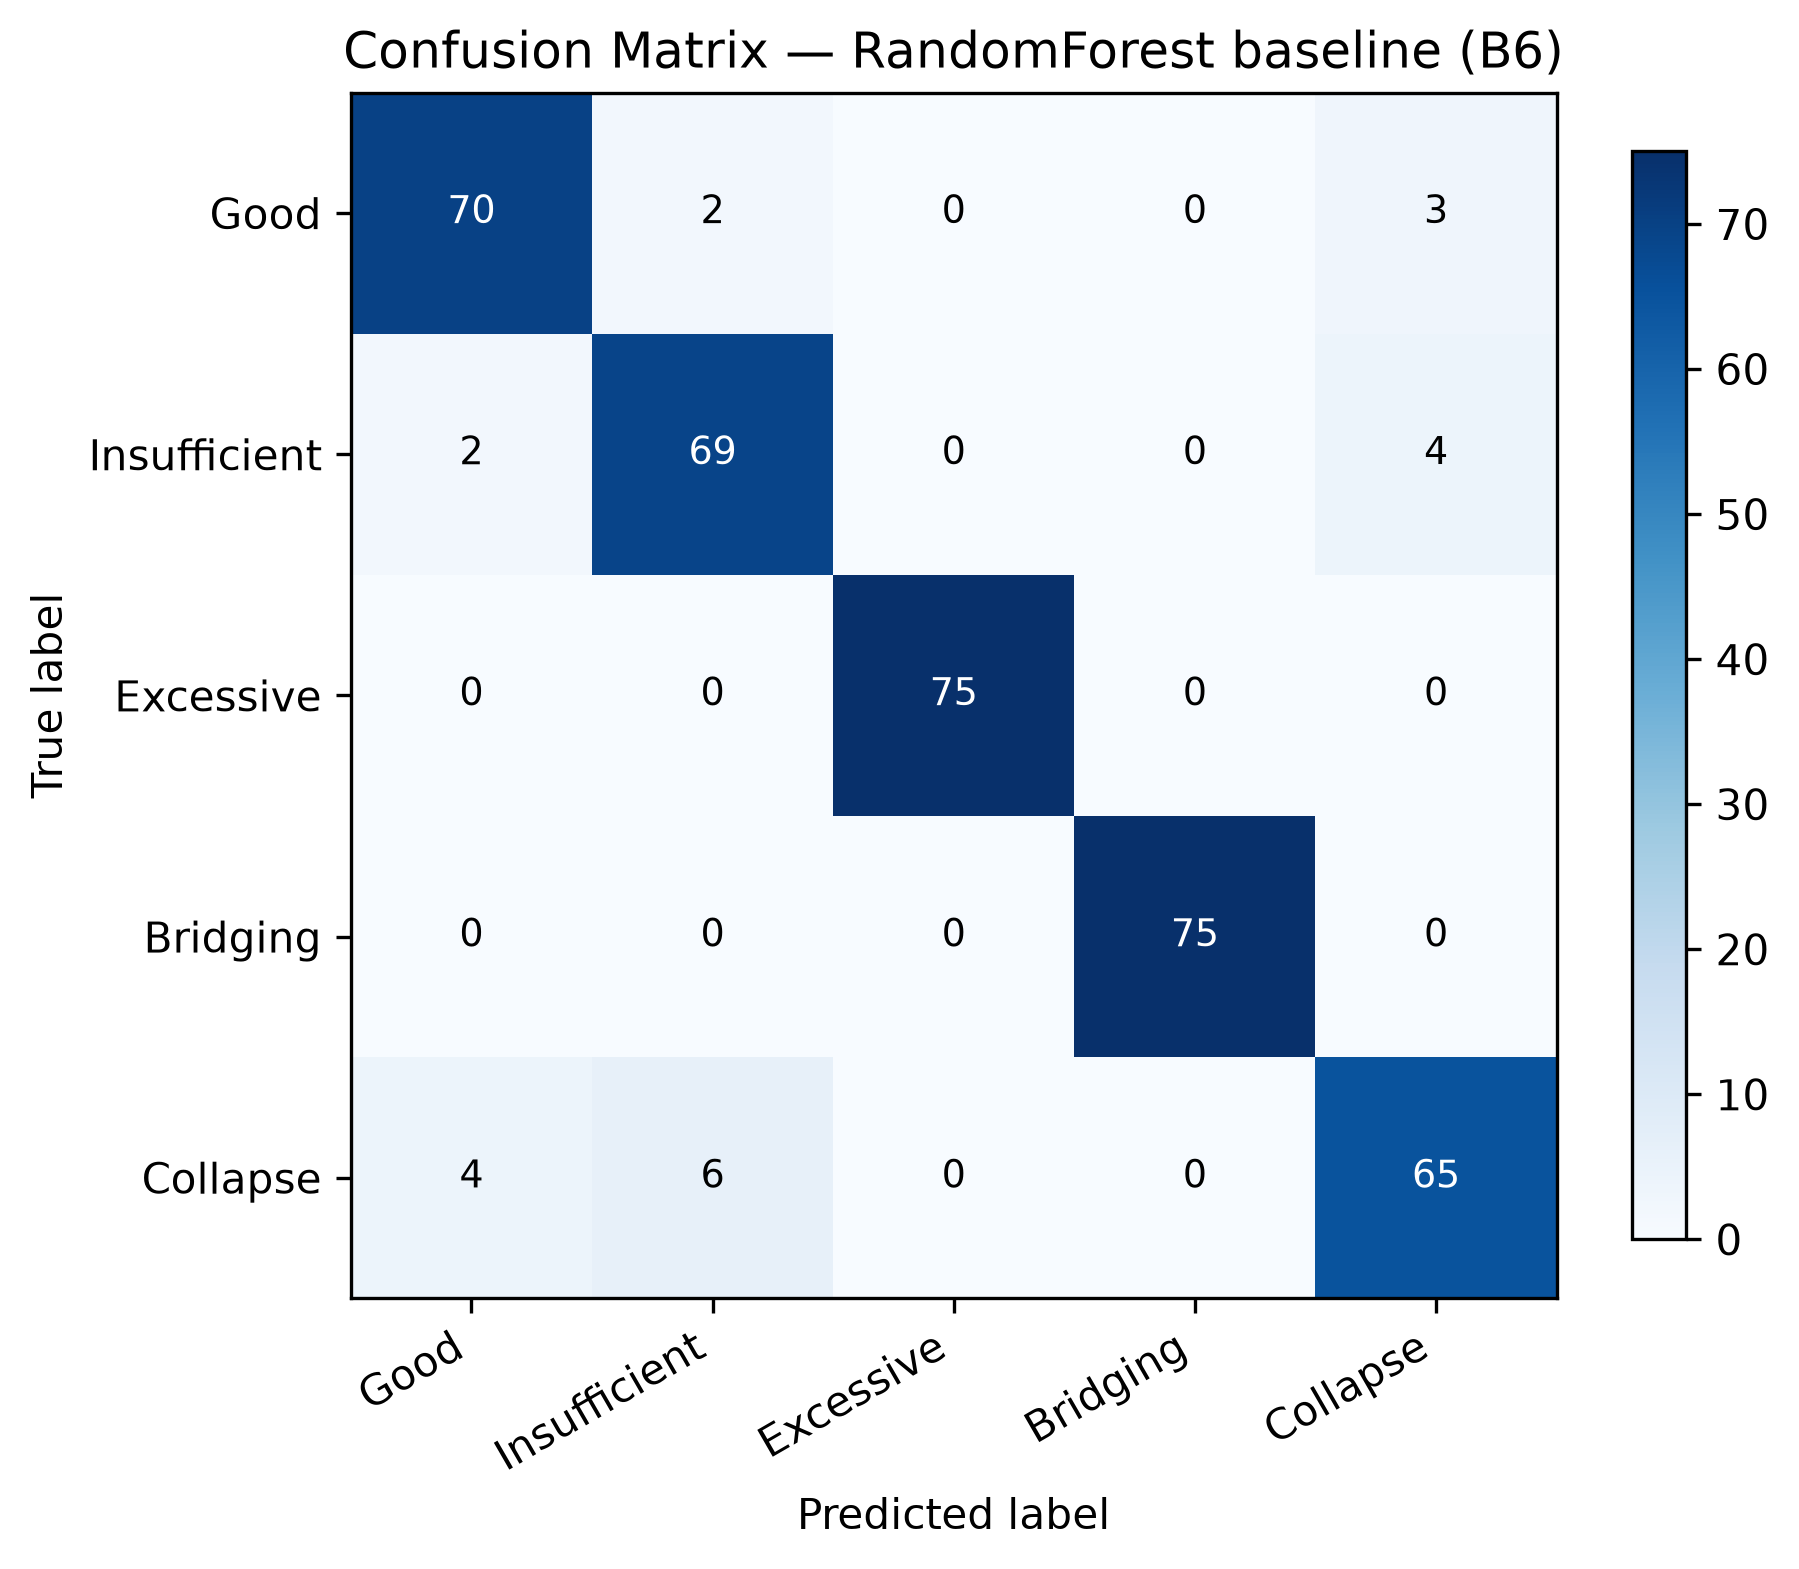
\includegraphics[width=0.34\textwidth]{fig1.png}
\caption{Confusion matrix for the Random Forest (B6) on the held-out test set (375 samples, seed = 42); the main confusion lies between collapse and the good and insufficient classes\DIFaddbeginFL \DIFaddFL{, while excessive solder incurs no test errors}\DIFaddendFL .}
\DIFaddbeginFL \label{fig:cm}
\DIFaddendFL \end{figure}
\DIFaddbegin 

\subsection{\DIFadd{Representative samples, robustness, and physical validity}}
\DIFadd{Figure~\ref{fig:samples} shows one representative synthetic point cloud per defect class (seed 42, 1500 points each). The generator is a parametric geometric model: every entry in Table~\ref{tab:params} has a physical interpretation --- the nominal joint radius $a$ and height $c$ set the joint scale in mm, }\texttt{\DIFadd{noise}} \DIFadd{is the sensor measurement standard deviation $\sigma$, and the shrinkage / inflation / bridging / collapse ranges express each defect as a controlled, physically meaningful deviation from the nominal geometry. This makes the benchmark's class difficulty directly tunable (widening the overlap ranges makes classes harder) and the defects interpretable, even though the clouds are not fitted to production scans.
}

\begin{figure}[htbp]
\centering
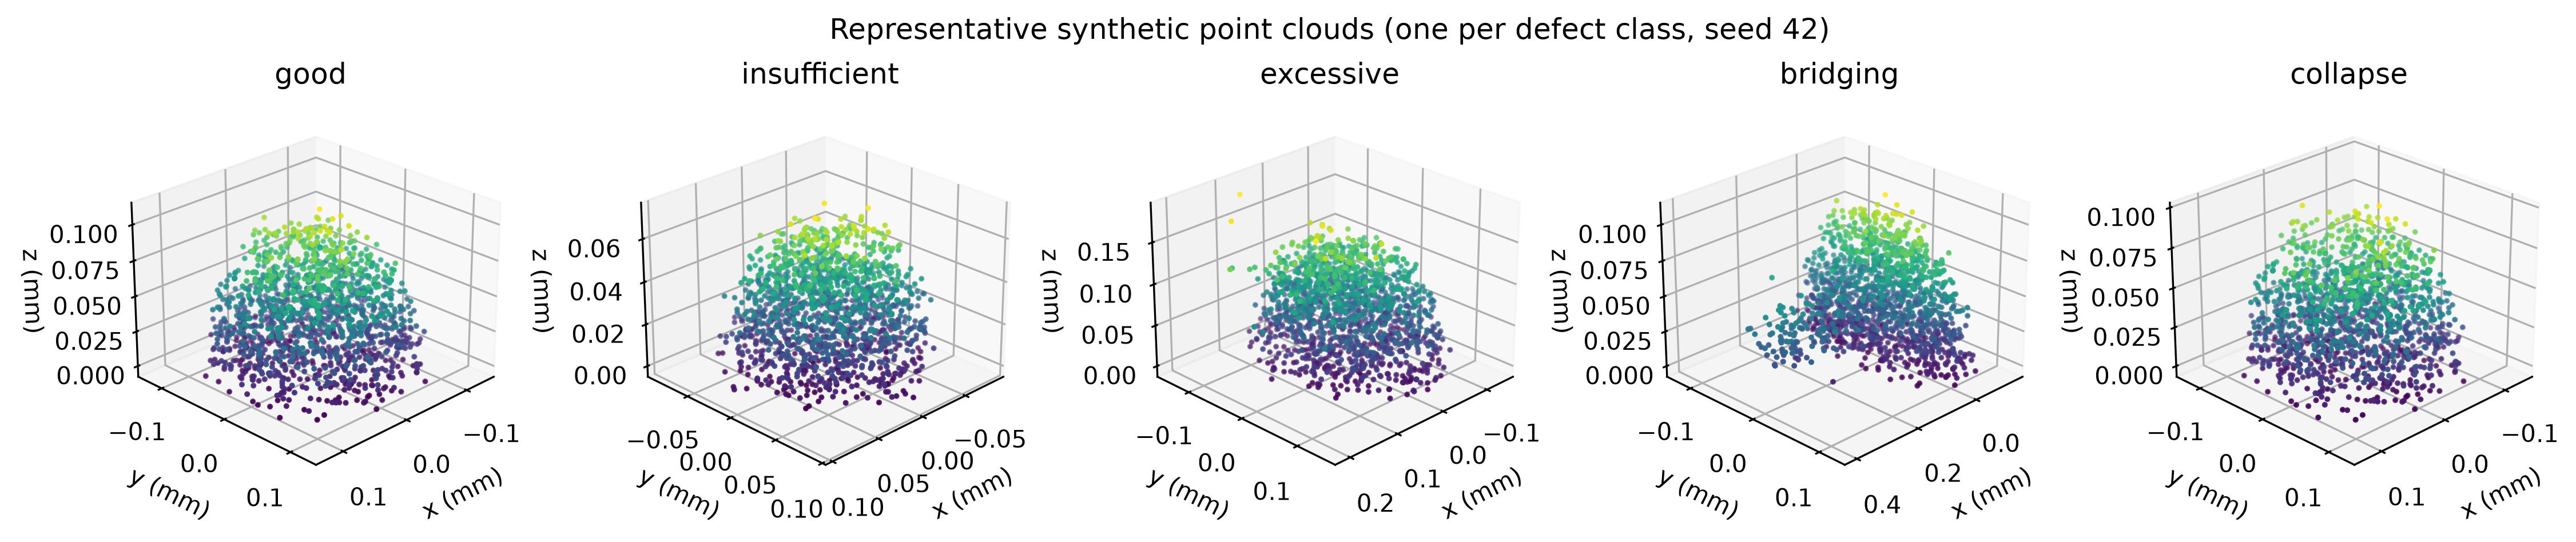
\includegraphics[width=0.92\linewidth]{sample_clouds.png}
\caption{\DIFaddFL{Representative synthetic point clouds, one per defect class (seed 42, 1500 points each; axes in mm). Good and insufficient differ mainly in scale; excessive adds a bump; bridging shows a low bridge to the neighbour; collapse shows a top dent.}}
\label{fig:samples}
\end{figure}

\begin{figure}[htbp]
\centering
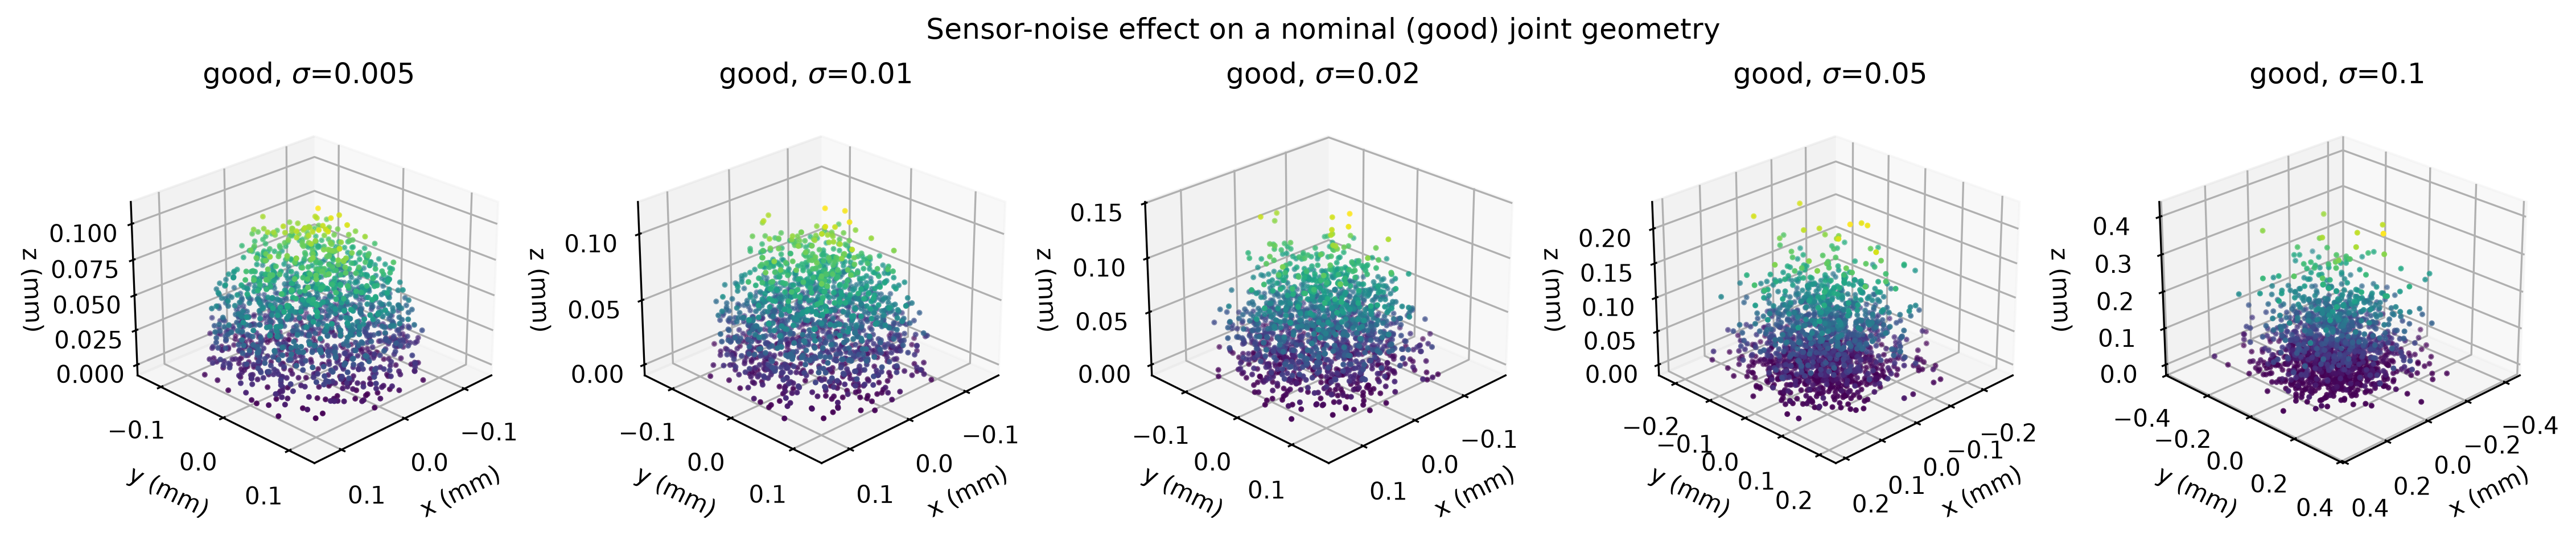
\includegraphics[width=0.92\linewidth]{noise_effect.png}
\caption{\DIFaddFL{Effect of sensor noise on a nominal (good) joint: as $\sigma$ grows the cloud becomes progressively rougher, degrading classifier accuracy (see Table~\ref{tab:noise}).}}
\label{fig:noise}
\end{figure}

\DIFadd{To verify that the reported ranking is not an artefact of a single configuration, we repeat the full comparison under varying sensor noise and defect-strength settings (seed 42). Table~\ref{tab:noise} varies the noise std.\ $\sigma$ over five levels $\sigma\in\{0.005,\allowbreak 0.01,\allowbreak 0.02,\allowbreak 0.05,\allowbreak 0.10\}$; accuracy falls monotonically and gracefully (RF 0.9440 $\to$ 0.7467) while the relative ordering of methods is preserved, confirming the benchmark is robust to sensor quality. Table~\ref{tab:defect} varies the class-overlap ranges: narrowing them (an easier task) raises RF accuracy to 0.9653, whereas widening them keeps RF at 0.9440 because the seven geometric features remain discriminative even under wide overlap --- i.e., difficulty is controllable in the easy direction and the features are robust to aggressive overlap. Together these ablations show the conclusions hold across a range of physically meaningful generator settings.
}

\begin{table}[htbp]
\centering
\caption{\DIFaddFL{Robustness to sensor noise. Accuracy of the random forest (B6), the S3DA rule (B1) and gradient boosting (B5), and the span of all six methods, as a function of the Gaussian noise std.\ $\sigma$ (seed 42).}}
\label{tab:noise}
\begin{tabular}{lcccc}
\toprule
\DIFaddFL{$\sigma$ }& \DIFaddFL{RF Acc. }& \DIFaddFL{S3DA Acc. }& \DIFaddFL{GB Acc. }& \DIFaddFL{Span$_{\mathrm{acc}}$ }\\
\midrule
\DIFaddFL{0.005 }& \DIFaddFL{0.9440 }& \DIFaddFL{0.5600 }& \DIFaddFL{0.9413 }& [\DIFaddFL{0.5600, 0.9440}] \\
\DIFaddFL{0.010 }& \DIFaddFL{0.9360 }& \DIFaddFL{0.5360 }& \DIFaddFL{0.9307 }& [\DIFaddFL{0.5360, 0.9387}] \\
\DIFaddFL{0.020 }& \DIFaddFL{0.9173 }& \DIFaddFL{0.4800 }& \DIFaddFL{0.9120 }& [\DIFaddFL{0.4800, 0.9307}] \\
\DIFaddFL{0.050 }& \DIFaddFL{0.8640 }& \DIFaddFL{0.2640 }& \DIFaddFL{0.8560 }& [\DIFaddFL{0.2640, 0.8827}] \\
\DIFaddFL{0.100 }& \DIFaddFL{0.7467 }& \DIFaddFL{0.2000 }& \DIFaddFL{0.7307 }& [\DIFaddFL{0.2000, 0.7547}] \\
\bottomrule
\end{tabular}
\end{table}

\begin{table}[htbp]
\centering
\caption{\DIFaddFL{Robustness to defect-strength / class-overlap configuration. RF accuracy and the worst-method accuracy under a narrow (easier), default, and wide (harder) overlap of the class parameter ranges (seed 42).}}
\label{tab:defect}
\begin{tabular}{lccc}
\toprule
\DIFaddFL{Configuration }& \DIFaddFL{RF Acc. }& \DIFaddFL{S3DA Acc. }& \DIFaddFL{Min acc. }\\
\midrule
\DIFaddFL{narrow (easier) }& \DIFaddFL{0.9653 }& \DIFaddFL{0.5760 }& \DIFaddFL{0.5760 }\\
\DIFaddFL{default }& \DIFaddFL{0.9440 }& \DIFaddFL{0.5600 }& \DIFaddFL{0.5600 }\\
\DIFaddFL{wide (harder) }& \DIFaddFL{0.9440 }& \DIFaddFL{0.5173 }& \DIFaddFL{0.5173 }\\
\bottomrule
\end{tabular}
\end{table}

\DIFaddend \subsection{Feature ablation}
Table~\DIFdelbegin \DIFdel{4 }\DIFdelend \DIFaddbegin \DIFadd{\ref{tab:loo} }\DIFaddend reports the leave-one-feature-out (LOO) ablation for the random forest (full-model macro-$F_1$ = 0.9439).
\begin{table}[htbp]
\centering
\caption{Leave-one-feature-out ablation of the RandomForest model (macro-$F_1$; full model = 0.9439).}
\DIFaddbeginFL \label{tab:loo}
\DIFaddendFL \begin{tabular}{lp{0.22\linewidth}p{0.50\linewidth}}
\toprule
\textbf{Removed feature} & \textbf{$\Delta F_1$ vs. full-model $F_1$} & \textbf{Interpretation} \\
\midrule
h\_var & -0.0459 & Most informative: collapse dents and excessive bumps reshape the height distribution \\
vol\_area\_ratio & -0.0105 & Compactness cue separating volumetric defects from nominal joints \\
min\_dist & -0.0054 & Small overall cost because bridging is nearly separable already \\
area & -0.0052 & Correlated with vol; adds modest independent signal \\
convex\_vol\_ratio & -0.0025 & Irregularity cue; partially redundant with h\_var \\
vol & +0.0026 & Slightly redundant once ratios are present \\
max\_h & 0.0000 & Fully redundant given h\_var and vol \\
\bottomrule
\end{tabular}
\end{table}
The ablation has a clean physical reading. Height variance (\texttt{h\_var}) is the single most valuable descriptor because the \DIFdelbegin \DIFdel{two hardest }\DIFdelend \DIFaddbegin \DIFadd{most error-prone }\DIFaddend defects --- collapse (a dent) and \DIFdelbegin \DIFdel{excessive solder (a bump}\DIFdelend \DIFaddbegin \DIFadd{insufficient solder (shrinkage}\DIFaddend ) --- \DIFdelbegin \DIFdel{are primarily height-distribution phenomena, whereas volume-only cues saturate}\DIFdelend \DIFaddbegin \DIFadd{primarily shift the height distribution, whereas excessive solder (a pronounced volume inflation) is in fact well separated, with zero test errors in Figure~\ref{fig:cm} because its volume signature is large and distinctive. Volume-only cues therefore saturate for the volumetric defects but miss the subtle height changes that distinguish collapse from good/insufficient}\DIFaddend . Single-feature runs corroborate this: the strongest single feature is \texttt{convex\_vol\_ratio} ($\text{macro-}F_1=0.6412$), which captures shape irregularity common to several defect types, while the weakest is \texttt{min\_dist} ($\text{macro-}F_1=0.3616$), which is highly informative for bridging but carries no signal for the other four classes. The near-zero or positive deltas for \texttt{vol} and \texttt{max\_h} indicate information redundancy rather than irrelevance: both are strongly correlated with the ratio features. Volume alone is in fact a \DIFdelbegin \DIFdel{strong }\DIFdelend \DIFaddbegin \DIFadd{useful but insufficient }\DIFaddend single cue --- it underpins the industrial S3DA rule (B1), which \DIFdelbegin \DIFdel{reaches 0.8960 accuracy using volume only }\DIFdelend \DIFaddbegin \DIFadd{thresholds volume only and reaches 0.5600 accuracy at seed 42 (0.5632 $\pm$ 0.0091 across seeds), i.e.\ well above chance but far below every learned model}\DIFaddend . Removing \texttt{vol} slightly increases macro-$F_1$ within small numerical fluctuations; this is purely a statistical artifact given that volume information is already encoded within ratio-based descriptors.
\begin{table}[htbp]
\centering
\caption{Selected representative single-feature macro-$F_1$ scores (RandomForest, seed = 42). Full results are programmatically exported by run\_ablation.}
\DIFaddbeginFL \label{tab:single}
\DIFaddendFL \begin{tabular}{lc}
\toprule
\textbf{Single feature} & \textbf{macro-$F_1$} \\
\midrule
\texttt{vol}               & 0.5494 \\
\texttt{max\_h}            & 0.5473 \\
\texttt{h\_var}            & 0.5808 \\
\texttt{area}              & 0.6409 \\
\texttt{vol\_area\_ratio}   & 0.5794 \\
\texttt{convex\_vol\_ratio} & 0.6412 \\
\texttt{min\_dist}         & 0.3616 \\
\bottomrule
\end{tabular}
\end{table}
\section{Impact}
Solderbench contributes to three communities. For inspection-algorithm research, it is the first public, reproducible 3D benchmark for solder-joint defect classification, replacing per-paper private datasets with a common task, protocol, and versioned reference numbers; new methods are ranked against six baselines with one command. For teaching, it is a self-contained geometric-ML case study that fits a short lab session and runs on any laptop, with each design decision doubling as a benchmark-methodology lesson. For reproducibility, seed-level determinism, a one-command script, machine-readable exports, a \texttt{codemeta.json} descriptor, and an MIT license make the software trivially citable, archivable, and reusable. The path to production data is short: a user with a real 3D AOI camera replaces the body of \texttt{load\_dataset} --- or passes their own X, y --- with code that reads scans, segments joints, and calls \texttt{extract\_features}; all downstream experiments run unchanged. Beyond the classical-ML workflow, the generator's raw point clouds can be passed directly to external deep models (e.g., PointNet \cite{ref8,ref9}); Solderbench supports both scenarios.
\section{Limitations}
We state the limitations of Solderbench honestly.
The generator is a geometric model, not a physics simulator: it does not model wetting dynamics, surface tension, oxidation, or realistic sensor artifacts (occlusion, multi-path reflections, structured-light failure); class distributions are plausible and overlapping, not fitted to production data. Three scope limits remain. First, the five classes are idealized single-fault geometries --- compound defects (e.g., insufficient and collapsed together) are unsupported, although they occur on real-world production lines. Second, the clouds model only the individual joint, omitting substrate, pads, and pins, so board-level context is out of scope. Third, resampling every cloud to a fixed $n_{\mathrm{points}}$ simplifies real sensors, which return a variable point-count, and may alter the point-density distribution. \DIFaddbegin \DIFadd{Finally, }\textbf{\DIFadd{all benchmark experiments reported in this manuscript are based exclusively on synthetic data}}\DIFadd{; the absolute accuracy values therefore cannot be directly transferred to industrial real-world inspection, and only the relative ordering of methods under a controlled, identical protocol should be read as a result.
}\DIFaddend \textbf{Consequently, Solderbench is suitable for algorithm prototyping, fair cross-method comparison, and descriptor-level analysis, but its metric values must not be read as predictions of real industrial AOI performance.} Synthetic validation cannot substitute for validation on real scans; the benchmark guarantees only that comparisons made on it are fair, controlled, and exactly reproducible --- a much-needed property currently missing from this research field.

%DIF <  Zenodo DOI 10.5281/zenodo.22959193 (release v0.1.1) filled in C3 and Data availability.
%DIF >  Zenodo concept DOI 10.5281/zenodo.22959192 (resolves to latest, v0.1.3); v0.1.1 version DOI 10.5281/zenodo.22959193 kept for reference.
\begin{sloppypar}\noindent\textbf{Data availability.} The Solderbench source code and all reproduction scripts are released under the MIT license and archived on Zenodo (\DIFdelbegin \DIFdel{doi:}\DIFdelend \DIFaddbegin \DIFadd{concept doi:}\url{10.5281/zenodo.22959192}\DIFadd{, version doi:}\DIFaddend \url{10.5281/zenodo.22959193} \DIFaddbegin \DIFadd{for v0.1.1}\DIFaddend ); the permanent GitHub repository is \url{https://github.com/wqinmin975/pcb}. The benchmark dataset is not stored as a fixed file but generated deterministically at runtime by running \texttt{python examples/run\_benchmark.py}, which regenerates every table and figure in this paper.\end{sloppypar}

\section{Conclusions}
We presented Solderbench, an open-source, pure-Python synthetic benchmark for 3D PCB solder-joint defect inspection with a parametric five-class generator, seed-level reproducibility, a seven-dimensional feature extractor, six baselines including the industrial S3DA rule, and automated comparison and ablation runners. On the reference benchmark (1250 samples, seed 42) a random forest reaches 0.9440 accuracy and 0.9439 macro-$F_1$. By removing the data-access barrier that fragments 3D solder-joint inspection, Solderbench makes development, comparison, and teaching open and reproducible. Future work: (i) fitting generator parameters to measured scans; (ii) adding sensor-artifact models; (iii) compound-defect taxonomy; (iv) real-data conversion scripts; (v) deep point-cloud model interfaces (e.g. PointNet, PointNet++); and (vi) preset difficulty templates.
\section{Acknowledgements}
This research did not receive any specific grant from funding agencies in the public, commercial, or not-for-profit sectors. Computations were performed with the Solderbench toolkit (MIT license).

\section*{Declaration of competing interest}
The authors declare that they have no known competing financial interests or personal relationships that could have appeared to influence the work reported in this paper.

\section*{CRediT authorship contribution statement}
\textbf{Qinmin Wang:} Conceptualization, Methodology, Software, Writing -- original draft.
\textbf{Zixin Wang:} Software, Validation, Data curation.
\textbf{Hongyuan Wang:} Resources, Supervision.
\textbf{Zongzhong Wang:} Writing -- review \& editing, Supervision, Project administration (Corresponding author).
\setlength{\bibsep}{0pt}
\begin{thebibliography}{17}\footnotesize
\bibitem{ref1}Q. Ling, N.A.M. Isa, Printed circuit board defect detection methods based on image processing, machine learning and deep learning: A survey, IEEE Access 11 (2023) 15921-15944. https://doi.org/10.1109/ACCESS.2023.3245093
\bibitem{ref2}Y. Zhou, M. Yuan, J. Zhang, G. Ding, S. Qin, Review of vision-based defect detection research and its perspectives for printed circuit board, Journal of Manufacturing Systems 70 (2023) 557-578. https://doi.org/10.1016/j.jmsy.2023.08.019
\bibitem{ref3}M. Moganti, F. Ercal, Automatic PCB inspection systems, IEEE Potentials 14(3) (1995) 6-10. https://doi.org/10.1109/45.464686
\bibitem{ref4}W. Dai, A. Mujeeb, M. Erdt, A. Sourin, Soldering defect detection in automatic optical inspection, Advanced Engineering Informatics 43 (2020) 101004. https://doi.org/10.1016/j.aei.2019.101004
\bibitem{ref5}S. Tang, F. He, X. Huang, J. Yang, Online PCB defect detector on a new PCB defect dataset, arXiv preprint arXiv:1902.06197 (2019). https://doi.org/10.48550/arXiv.1902.06197
\bibitem{ref6}Y. Xu, Z. Wang, J. Liang, Y. Zhang, J. Feng, W. Miao, J. Wang, G. Pu, S3DA: A 3D point cloud based PCB solder defect detection algorithm, in: S. Liu (Ed.), Software Fault Prevention, Verification, and Validation (SFPVV 2024), Lecture Notes in Computer Science, vol. 15393, Springer, 2025, pp. 115-130. https://doi.org/10.1007/978-981-96-1621-3\_8
\bibitem{ref7}Q. Hu, K. Hao, B. Wei, H. Li, An efficient solder joint defects method for 3D point clouds with double-flow region attention network, Advanced Engineering Informatics 52 (2022) 101608. https://doi.org/10.1016/j.aei.2022.101608
\bibitem{ref8}C.R. Qi, H. Su, K. Mo, L.J. Guibas, PointNet: Deep learning on point sets for 3D classification and segmentation, in: Proceedings of the IEEE Conference on Computer Vision and Pattern Recognition (CVPR), 2017, pp. 652-660. https://doi.org/10.1109/CVPR.2017.16
\bibitem{ref9}C.R. Qi, L. Yi, H. Su, L.J. Guibas, PointNet++: Deep hierarchical feature learning on point sets in a metric space, in: Advances in Neural Information Processing Systems 30 (NeurIPS), 2017, pp. 5099-5108. https://proceedings.neurips.cc/paper/2017/hash/d8bf84be3800d12f74d8b05e9b89836f-Abstract.html
\bibitem{ref10}Q.-Y. Zhou, J. Park, V. Koltun, Open3D: A modern library for 3D data processing, arXiv preprint arXiv:1801.09847 (2018). https://arxiv.org/abs/1801.09847
\bibitem{ref11}L. Breiman, Random forests, Machine Learning 45(1) (2001) 5-32. https://doi.org/10.1023/A:1010933404324
\bibitem{ref12}C. Cortes, V. Vapnik, Support-vector networks, Machine Learning 20(3) (1995) 273-297. https://doi.org/10.1007/BF00994018
\bibitem{ref13}F. Pedregosa, G. Varoquaux, A. Gramfort, V. Michel, B. Thirion, O. Grisel, M. Blondel, P. Prettenhofer, R. Weiss, V. Dubourg, J. Vanderplas, A. Passos, D. Cournapeau, M. Brucher, M. Perrot, E. Duchesnay, Scikit-learn: Machine learning in Python, Journal of Machine Learning Research 12 (2011) 2825-2830.
\bibitem{ref14}C.R. Harris, K.J. Millman, S.J. van der Walt, R. Gommers, P. Virtanen, D. Cournapeau, E. Wieser, J. Taylor, S. Berg, N.J. Smith, et al., Array programming with NumPy, Nature 585 (2020) 357-362. https://doi.org/10.1038/s41586-020-2649-2
\bibitem{ref15}P. Virtanen, R. Gommers, T.E. Oliphant, M. Haberland, T. Reddy, D. Cournapeau, E. Burovski, P. Peterson, W. Weckesser, J. Bright, et al., SciPy 1.0: Fundamental algorithms for scientific computing in Python, Nature Methods 17 (2020) 261-272. https://doi.org/10.1038/s41592-019-0686-2
\bibitem{ref16}W. McKinney, Data structures for statistical computing in Python, in: Proceedings of the 9th Python in Science Conference, 2010, pp. 51-56. https://doi.org/10.25080/Majora-92bf1922-00a
\bibitem{ref17}J.D. Hunter, Matplotlib: A 2D graphics environment, Computing in Science \& Engineering 9(3) (2007) 90-95. https://doi.org/10.1109/MCSE.2007.55
\end{thebibliography}
\end{document}
